\chapter{Introduction}
\writer{Ties Behnke, Kiyotomo Kawagoe}{2}
The ILD detector is a proposed detector for the international linear collider, ILC. It has been developed over the last 10 years within a proto-collaboration with the goal to develop and eventually propose a fully integrated detector for the ILC. 

The fundamental ideas and concepts behind the ILD detector have been discussed in two previous documents, the letter of intent \cite{ild:bib:ILDloi} and the detailed baseline document, DBD \cite{ild:bib:ILDDBD}. This document summarises the overall design of the detector, describes developments since the publishing of the DBD, and describes in more detail an effort to optimize the ILD detector. 

The ILD detector concept has been designed as a multi-purpose detector. It should deliver excellent physics performance for collision energies between 90~Gev and 1~TeV, the largest possible energy reach of the ILC. The ILD detector has been optimized to perform excellently at the initial ILC energy of 250 GeV. 

The science which will be done at the ILC requires a true multi-purpose detector. A central element of the design has been the capability of the detector to reconstruct precisely complex hadronic final states as well as more events with leptons or missing energy in the final state. Thus traditional precision detector elements as vertex detectors are combined in an overall design philosophy called particle flow, which has been developed for optimal hadronic event reconstruction.

The high precision vertex detector positioned very closely to the interaction point is followed by a hybrid tracking layout, realised as a combination of silicon tracking with a time projection chamber, and a calorimeter system. The complete system is located inside a large solenoid providing a magnetic field of 3.5-4 T. On the outside of the coil, the iron return yoke is instrumented as a muon system and as a tail catcher calorimeter. 
	
\thisfloatsetup{floatwidth=\SfigwFull,capposition=beside}
\begin{figure}[b!]
\begin{tabular}{cc}

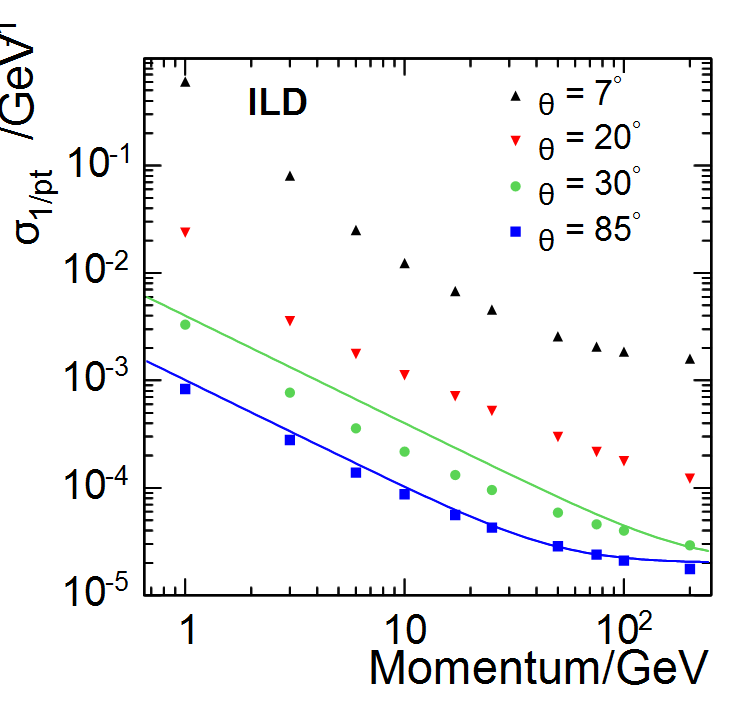
\includegraphics[width=0.5\hsize]{Introduction/fig/deltaInvP_all_fits.png} &
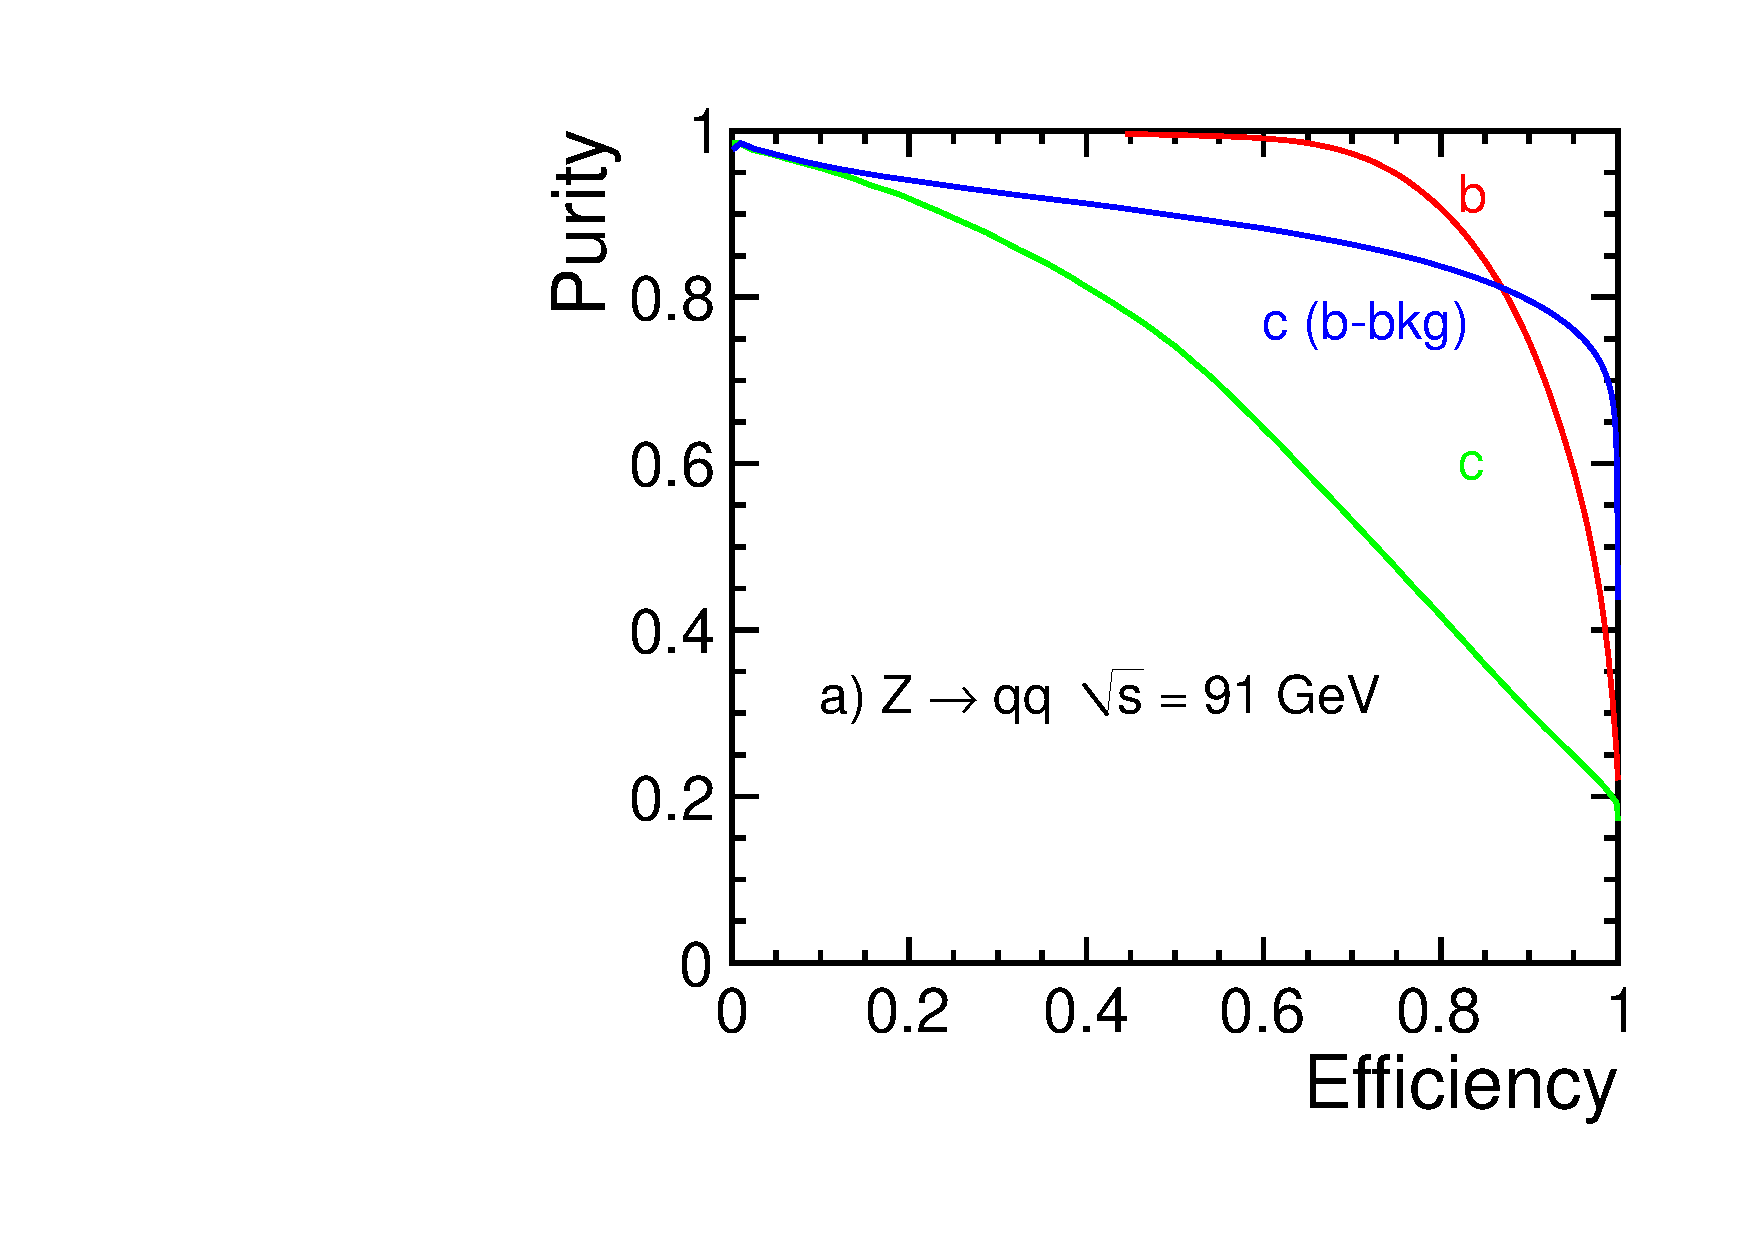
\includegraphics[width=0.5\hsize]{Introduction/fig/evalZ-lcfiweights_qq91new_v02-test.pdf}
\end{tabular}
\caption{\label{ild:fig:intro:tracking}(left) Momentum resolution for the ILD detector concept, as a function of the transverse momentum of the particle. (right) Flavour tagging efficiency versus purity for bottom events in sample of Z decays at 91\,GeV, and for charm events with only bottom background. )}
\end{figure}



\begin{figure}[t!]

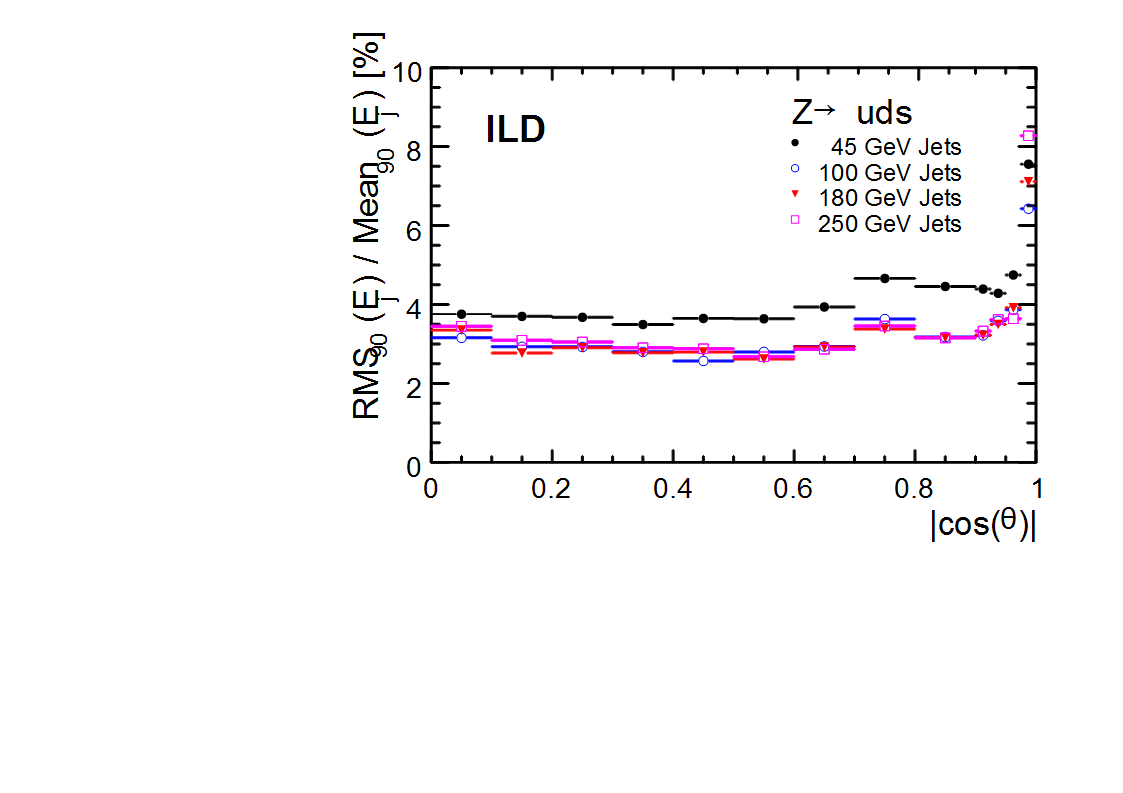
\includegraphics[width=0.8\hsize]{Introduction/fig/ild01_o1_pflow.png}

\caption{\label{ild:fig:intro:pflow}Fractional jet energy resolution
    plotted against $|\cos\theta|$ where theta is the polar angle of the thrust axis of the event. }
\end{figure}

The performance of the ILD concept has been extensively studied using a detailed GEANT4 based simulation model and sophisticated reconstruction tools. Backgrounds have been taken into account to the best of current knowledge.

The performance of the tracking system can be summarised by its combined momentum resolution, shown in Figure~\ref{ild:fig:intro:tracking}~(left). A resolution of $\sigma_{1/p_T} = 2 \times 10^{-5}$\,GeV$^{-1}$ has been achieved for high momenta. For many physics studies the tagging of long lived particles is of key importance. Several layers of pixel detectors close to the IP allow the reconstruction of displaced vertices, as shown in Figure~\ref{ild:fig:intro:tracking}~(right).

Calorimeter system and tracking system together enter into the particle flow performance. The performance of the ILD detector for different energies and as a function of the polar angle is shown in Figure~\ref{ild:fig:intro:pflow}. 

The few plots shown in this introduction illustrate the anticipated performance of the detector and illustrate the potential for precision measurements with the ILD detector. More details on the performance may be found in section~\ref{ild:sec:performance} of this document. 

In this document the current state of the design of the ILD detector is summarised. The technologies which are proposed for the different parts of the detector are introduced. An extensive benchmarking has been performed, to demonstrate the performance of the ILD detector. This has been done for two different detector implementations, a large and a smaller one. Both concepts are the result of intense optimization efforts, with different goals - cost effectivnes was foremost a criterium for the smaller one, ultimate performance for the larger model. 

The ILD group who is proposing this detector has currently some 70 member institutes from all around the world. The group has evolved into a proto-collaboration, which is positioning itself to move forward with a proposal for a detector at the ILC at the moment that ILC becomes a real project. 

A lot of the work presented in this report is based on intense R\&D work which has taken place over the last decade to develop the necessary technologies. 
This work has typically happened within dedicated R\&D collaborations, which are independent but maintain very close connections to ILD. All technologies selected by ILD for one of its subsystems have been proven experimentally to meet the performance goals, or to come very close. 

Developing a very powerful detector concept over a long period of time requires balancing cutting edge technologies, which might become available while the concept is being developed, with safe and sound solutions. ILD in many cases is pursuing more than one technological option, to remain flexible and to be able to adopt to new developments. The concept group  wants to remain open and flexible to be prepared to select the most modern and most powerful technology once it is necessary. 
However a distinction is made between options and alternatives: while options have undergone an extensive R\&D program and have passed critical proof-of-concept tests, alternatives are potentially interesting and promising technologies which have not matured to a similar level at the time of writing this document. 

The document starts with a short review of the science goals of the ILC, and how the goals can be achieved today with the detector technologies at hand. After a discussion of the ILC and the environment in which the experiment will take place the detector is described in more detail. The integration of the different sub-systems into an integrated detector is discussed, as is the interface between the detector and the collider. This is followed by a concise summary of the benchmarking which has been performed in order to find an optimal balance between performance and cost. To this end the costing methodology used by ILD is presented, and a cost estimate for the detector in 2018 costs is presented. The report closes with a summary of the proposed detector and its performance. 